\documentclass[12 pt]{article}

\usepackage{stoversymb}
\usepackage{fullpage,amsmath,amsfonts,amssymb,url,multicol,graphicx,tikz,soul}
%===makes urls render well===
\usepackage{lmodern}
\usepackage[T1]{fontenc}
%============================
\usepackage{wasysym} % smileys
\usepackage[inline]{enumitem}

\everymath{\displaystyle}

%\setenumerate{itemsep=0.25in}
\setlist[enumerate,1]{label=\arabic*., itemsep=0.375in}
\setlist[enumerate,2]{label={(\alph*)}, itemsep=0.3125in}
\setlist[enumerate,3]{label={\roman*.}}

\newcommand{\truefalse}[1]{#1\hfill\rule[-1mm]{220pt}{0.75pt}}
\newcommand{\hint}[1]{(\textbf{Hint}: #1)}
\newcommand{\note}[1]{\textbf{Note}: #1}
\newcommand{\infsum}[3]{\sum_{{#1}={#2}}^\infty {#3}}
\newcommand{\axes}[1]{\begin{center}
\includegraphics[scale=#1]{3DAxes}\end{center}}
\newcommand{\comps}[1]{\langle #1_1,#1_2,#1_3\rangle}
\newcommand{\compslong}[3]{\langle #1, #2, #3\rangle}
\newcommand{\ijk}[2]{#1\vect{#2}}

\graphicspath{ {./../img/} }
\DeclareGraphicsExtensions{.pdf}

\begin{document}
\begin{flushright}Name: \line(1,0){200}\end{flushright}
\begin{center}
\Large{\textbf{MAC 2313 --- Homework 1}}
\end{center}
\textbf{Directions:} Complete the following problems for a homework grade. Solutions \textit{must} be presented in a neat and professional manner in order to receive credit, answers given without showing work will not be eligible to receive partial credit, and \textit{work for the problems \textbf{must} be done on scratch paper and not on this handout!} \textbf{Date Due:} Monday, January 30.
\vspace{0.125in}
\begin{enumerate}[leftmargin=0in, rightmargin=-0.25in]
	%========Slack==============
	\item 
	\begin{enumerate}[itemsep=0.125in]
		\item Navigate to our course homepage at
		\begin{center} \url{http://www.math.fsu.edu/~cstover/teaching/sp17_2313/}
		\end{center}
		\item Read and familiarize yourself with the three resources listed under \textit{Supplementary Resources} on the \textsc{General Info} tab.
		\item Follow the instructions for using \textsc{Slack} messenger.\begin{quote}\textbf{Note:} This may require that I approve your email address, so to avoid some last minute glitch where I don't get to your approval on-time, please don't wait to do this!\end{quote}
		\item Navigate to the channel \url{#random} in the left column under \textsc{Channels} (its browser url should be something like \url{https://spring2017-calc3.slack.com/messages/random/}) and introduce yourself.\begin{quote}\textbf{Note:} This will be visible to everyone who signs into our class's chat room, so you definitely want to keep this PG-13, safe for work, and non-incriminatory. {\Large\smiley}\end{quote}
	\end{enumerate}\vspace{-0.125in}
	
	\item Plot $(1,-1,1)$ and $\langle -2,2,-3\rangle$ on the axes provided below. \note{The arrowheads are pointing towards the \textit{positive} values on each axis!}
	\axes{0.333}

	\item Write the vector from $(0,1,2)$ to $(1,\pi,-4)$ in terms of the standard basis vectors $\vect{i}$, $\vect{j}$, and $\vect{k}$.
	
	\item Consider the vectors $\vect{u}=\langle -2,3,1\rangle$, $\vect{v}=\vect{i}+\vect{j}+\vect{k}$, and $\vect{w}=\langle 0,-1,-1 \rangle$. Determine whether each of the following quantities is a scalar or a vector, and express each vector with respect to $\vect{i}$, $\vect{j}$, and $\vect{k}$.
	%\begin{multicols}{2}
	\begin{enumerate}
		\item $\vect{v}+\vect{w}$
		\item $3\vect{v}$
		\item $\left(\vect{u}\cdot\vect{w}\right)\vect{v}$
		\item The unit vector in the same direction as $\vect{u}+\vect{w}$
		\item $\left(\vect{w}\cdot\vect{w}\right)\vect{w}$
		\item $\vect{w}\times\vect{u}$
		\item $\vect{u}\times\vect{w}$
		\item The angle between $\vect{u}+\vect{w}$ and $\vect{u}\times\vect{w}$.
		\item The unit vector in the same direction as $\vect{w}\times\vect{u}-\vect{u}\times\vect{w}$
		\item $|\vect{v}-\vect{w}|$
		\item $|\vect{v}\times\vect{u}|$
		\item The unit vector orthogonal to both $\vect{u}+3\vect{v}$ and $2\vect{w}$
		\item The area of the parallelogram spanned by $\vect{u}+\vect{i}$ and $-2\vect{w}$
		\item $\comp_{\vect{u}}\vect{v}$ and $\proj_{\vect{u}}\vect{v}$ 
	\end{enumerate}

%	\item Describe the regions in $\Reals^3$ represented by each of the following. Give as much detail as possible (e.g. what're the center/radius of the sphere? what coordinate plane is the plane parallel to? etc.)
%	\begin{enumerate}
%		\item $3x^2+3y^2+3z^2=10+6y+12z$
%		\item $z=x$
%		
%	\end{enumerate}
	\item Let $\vect{a}=\langle a_1,a_2,a_3\rangle$, $\vect{b}=\langle b_1,b_2,b_3\rangle$, $\vect{c}=\langle c_1,c_2,c_3\rangle$, $\vect{u}=\langle u_1,u_2,u_3\rangle$, and $\vect{v}=\langle v_1,v_2,v_3\rangle$ be arbitrary vectors in $\Reals^3$. Prove each of the following.
	\begin{enumerate}[itemsep=0.95in]
		\item $\vect{i}\cdot\vect{j}=\vect{j}\cdot\vect{k}=\vect{k}\cdot\vect{i}=0$
		\item $\vect{i}\cdot\vect{i}=\vect{j}\cdot\vect{j}=\vect{k}\cdot\vect{k}=1$
		\item The vector $\vect{b}-\proj_{\vect{a}}\vect{b}$ is orthogonal to $\vect{a}$
		\item $|\vect{a}+\vect{b}|^2+|\vect{a}-\vect{b}|^2=2|\vect{a}|^2+2|\vect{b}|^2$
		\item $\vect{a}\times(\vect{b}\times\vect{c})=(\vect{a}\cdot\vect{c})\vect{b}-(\vect{a}\cdot\vect{b})\vect{c}$
		\item $(\vect{u}\times\vect{v})\cdot(\vect{a}\times\vect{b})=(\vect{u}\cdot\vect{a})(\vect{v}\cdot\vect{b})-(\vect{v}\cdot\vect{a})(\vect{u}\cdot\vect{b})$
		\item $(\vect{u}\times\vect{v})\times\vect{w}+(\vect{v}\times\vect{w})\times\vect{u}+(\vect{w}\times\vect{u})\times\vect{v}=\vect{0}$
	\end{enumerate}
	
	\newpage
	
	\item Find each of the following.
	\begin{enumerate}
		\item The equation of the line passing through $(2,1,-3)$ and $(6,-1,-5)$.
		\item The equation of the line passing through $(3,-1,2)$ in the direction of $\ijk{2}{i}-\ijk{3}{j}+\ijk{4}{k}$.
		\item The equation of the line through $(1,-1,4)$ and perpendicular to both $\vect{i}+\vect{j}-\vect{k}$ and $\compslong{0}{-3}{4}$.
		\item The equation of the plane passing through $(1,1,1)$ with normal vector $\vect{n}=\ijk{2}{i}+\ijk{}{j}-\ijk{2}{k}$.
		\item A unit normal vector to the plane $3x+y-z=10$.
		\item The equation of the plane through the point $(3,-1,-1)$ and perpendicular to the vector $\ijk{}{i}-\ijk{2}{j}+\ijk{}{k}$.
		\item The equation of the line through $(1,1,1)$ and orthogonal to the plane containing $(0,1,0)$, $(1,0,0)$, and $(0,0,1)$.
		\item The angle between the planes $x+y+z=1$ and $-x-6y+z=4$.
		\item The (curve formed by the) intersection of the two-sheet hyperboloid $-x^2+\frac{1}{4}y^2-\frac{1}{2}z^2=1$ and the plane $z=x-\frac{1}{10}y$ (see figures below).  \textbf{Simplify fully!}
	\end{enumerate}
	\vfill
	\begin{center}
		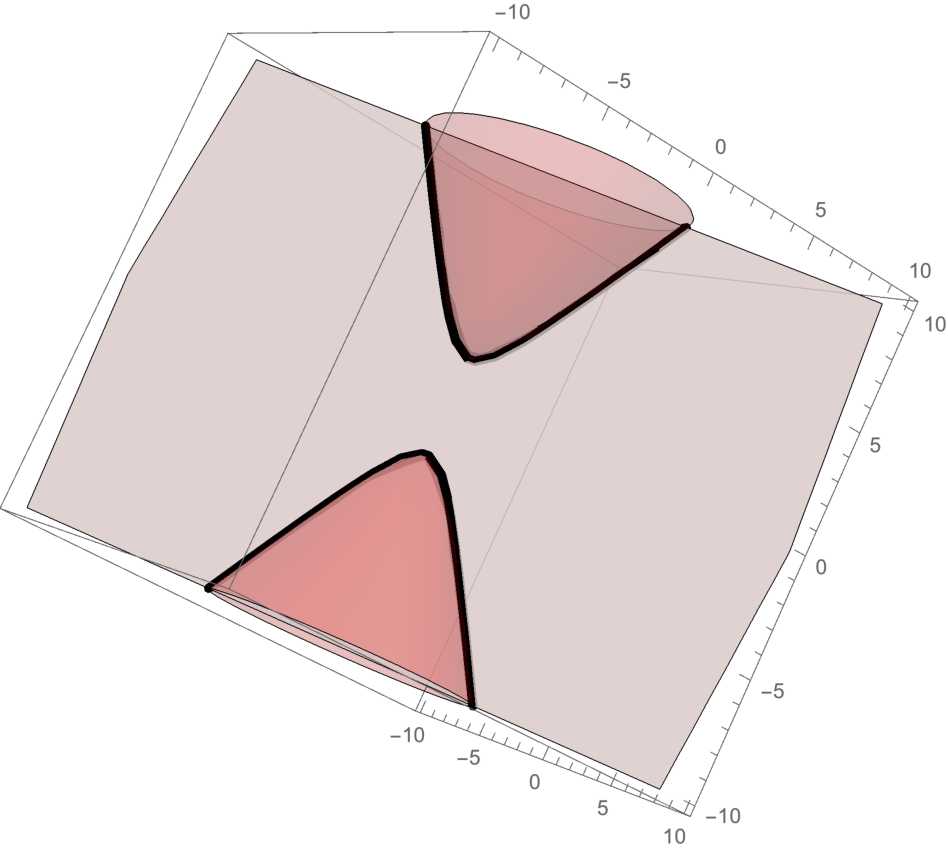
\includegraphics[scale=0.44]{PlaneHyperboloid}\hspace{1in}
		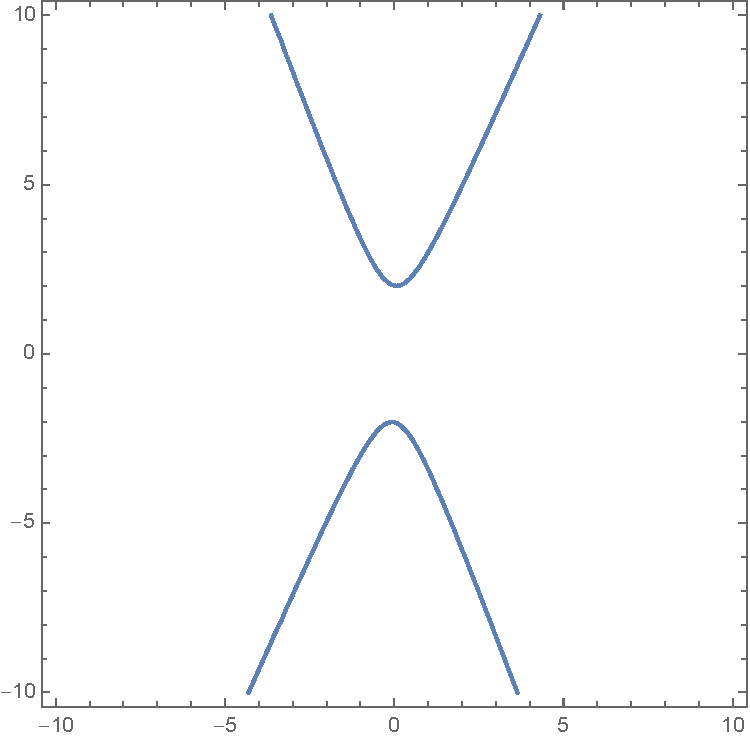
\includegraphics[scale=0.45]{PlaneHyperboloid2}
	\end{center}
\end{enumerate}
\end{document}